%%%%%%%%%%%%%%%%%%%%%%%%%%%%%%%%%%%%%%%%%
% Arsclassica Article
% LaTeX Template
% Version 1.1 (1/8/17)
%
% This template has been downloaded from:
% http://www.LaTeXTemplates.com
%
% Original author:
% Lorenzo Pantieri (http://www.lorenzopantieri.net) with extensive modifications by:
% Vel (vel@latextemplates.com)
%
% License:
% CC BY-NC-SA 3.0 (http://creativecommons.org/licenses/by-nc-sa/3.0/)
%
%%%%%%%%%%%%%%%%%%%%%%%%%%%%%%%%%%%%%%%%%

%----------------------------------------------------------------------------------------
%	PACKAGES AND OTHER DOCUMENT CONFIGURATIONS
%----------------------------------------------------------------------------------------
\documentclass[
11pt, % Main document font size
a4paper, % Paper type, use 'letterpaper' for US Letter paper
oneside, % One page layout (no page indentation)
%twoside, % Two page layout (page indentation for binding and different headers)
headinclude,footinclude, % Extra spacing for the header and footer
BCOR5mm, % Binding correction
]{scrartcl}

% configuration file where all the packages are loaded and set up
% commands new/redefined are done in here
%%%%%%%%%%%%%%%%%%%%%%%%%%%%%%%%%%%%%%%%%
% Arsclassica Article
% Structure Specification File
%
% This file has been downloaded from:
% http://www.LaTeXTemplates.com
%
% Original author:
% Lorenzo Pantieri (http://www.lorenzopantieri.net) with extensive modifications by:
% Vel (vel@latextemplates.com)
%
% License:
% CC BY-NC-SA 3.0 (http://creativecommons.org/licenses/by-nc-sa/3.0/)
%
%%%%%%%%%%%%%%%%%%%%%%%%%%%%%%%%%%%%%%%%%

%----------------------------------------------------------------------------------------
%	REQUIRED PACKAGES
%----------------------------------------------------------------------------------------

\usepackage[
nochapters, % Turn off chapters since this is an article        
beramono, % Use the Bera Mono font for monospaced text (\texttt)
eulermath,% Use the Euler font for mathematics
pdfspacing, % Makes use of pdftex’ letter spacing capabilities via the microtype package
dottedtoc % Dotted lines leading to the page numbers in the table of contents
]{classicthesis} % The layout is based on the Classic Thesis style

\usepackage{url} % Allows usage of hyperlinks
\usepackage{arsclassica} % Modifies the Classic Thesis package
\usepackage[T1]{fontenc} % Use 8-bit encoding that has 256 glyphs
\usepackage[utf8]{inputenc} % Required for including letters with accents
\usepackage[swedish, english]{babel}
\usepackage{graphicx} % Required for including images
\usepackage{enumitem} % Required for manipulating the whitespace between and within lists
\usepackage{lipsum} % Used for inserting dummy 'Lorem ipsum' text into the template
\usepackage{subfig} % Required for creating figures with multiple parts (subfigures)
\usepackage{amsmath,amssymb,amsthm} % For including math equations, theorems, symbols, etc
\usepackage{varioref} % More descriptive referencing

\usepackage[pages=some, scale=1, angle=0, opacity=0.7]{background}
\backgroundsetup{
  contents={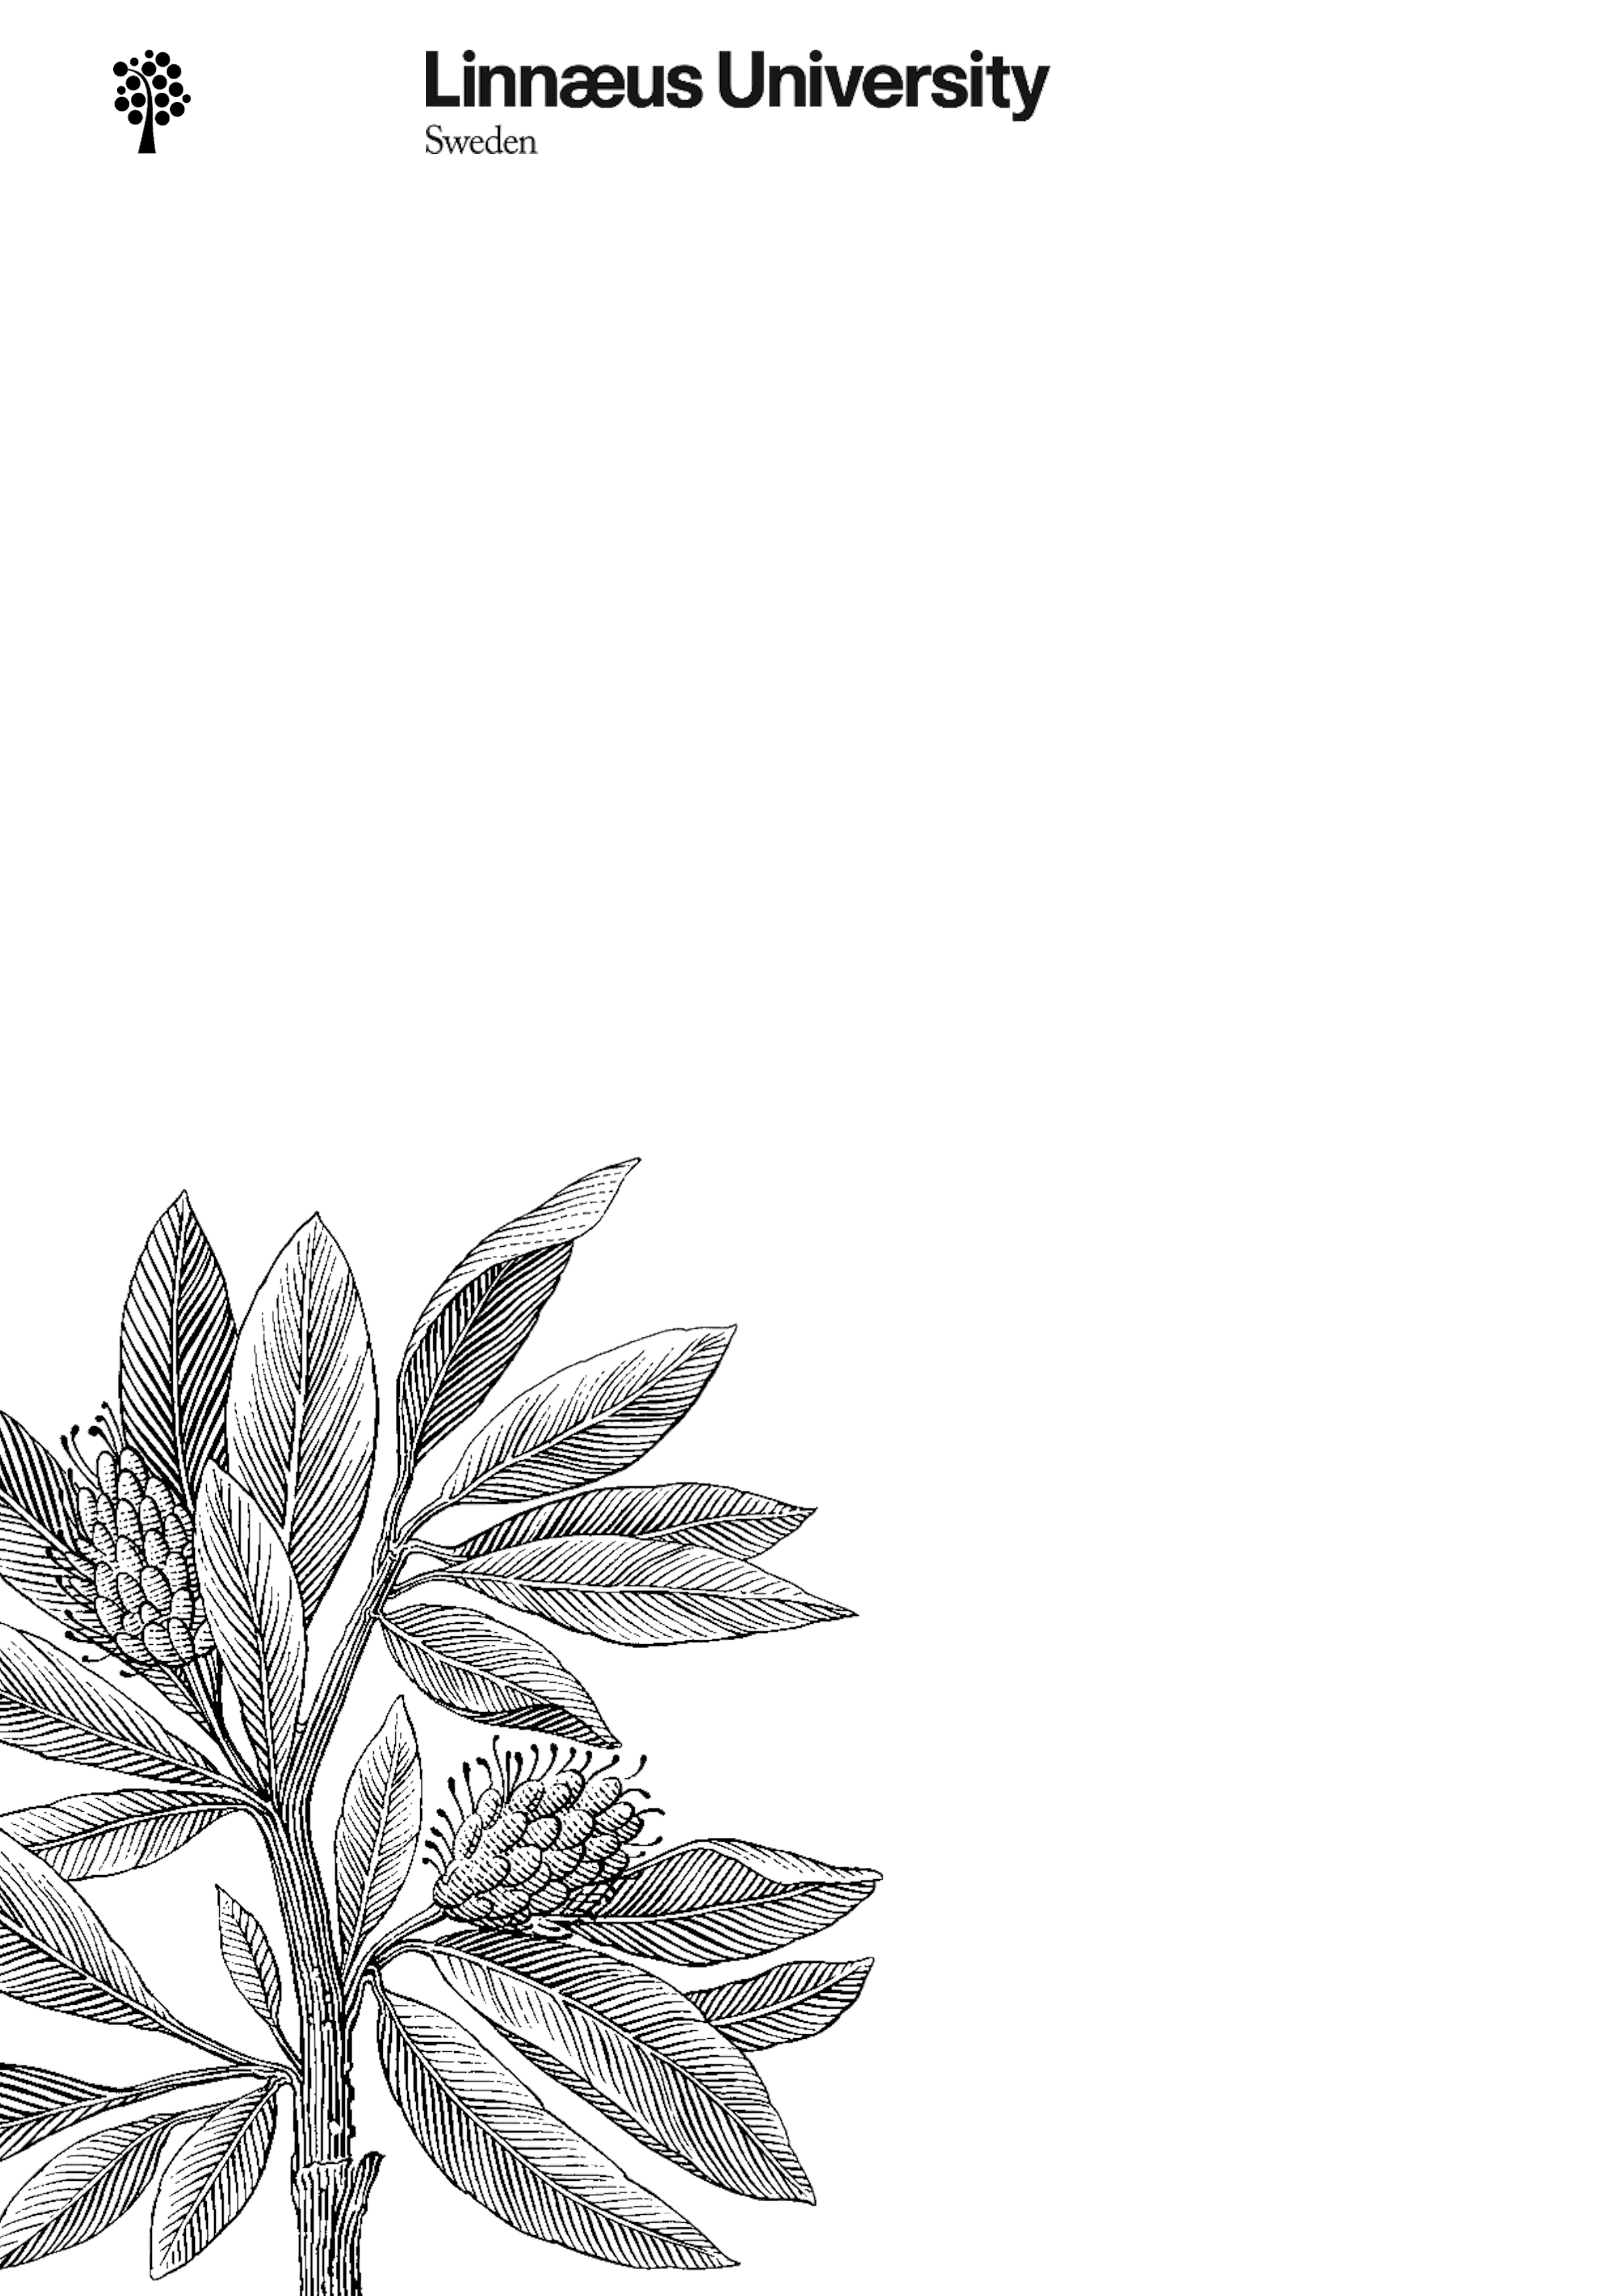
\includegraphics{titlepage_background}}
}
\usepackage{xcolor}

\usepackage{geometry}

\graphicspath{{logo/},{figures/}} % Set the default folder for images
%----------------------------------------------------------------------------------------
%	THEOREM STYLES
%---------------------------------------------------------------------------------------

\theoremstyle{definition} % Define theorem styles here based on the definition style (used for definitions and examples)
\newtheorem{definition}{Definition}

\theoremstyle{plain} % Define theorem styles here based on the plain style (used for theorems, lemmas, propositions)
\newtheorem{theorem}{Theorem}

\theoremstyle{remark} % Define theorem styles here based on the remark style (used for remarks and notes)

%----------------------------------------------------------------------------------------
%	HYPERLINKS
%---------------------------------------------------------------------------------------

\hypersetup{
%draft, % Uncomment to remove all links (useful for printing in black and white)
colorlinks=true, breaklinks=true, bookmarks=true,bookmarksnumbered,
urlcolor=webbrown, linkcolor=RoyalBlue, citecolor=webgreen, % Link colors
pdftitle={}, % PDF title
pdfauthor={\textcopyright}, % PDF Author
pdfsubject={}, % PDF Subject
pdfkeywords={}, % PDF Keywords
pdfcreator={pdfLaTeX}, % PDF Creator
pdfproducer={LaTeX with hyperref and ClassicThesis} % PDF producer
}



\newcommand*{\reporttitle}[1]{\def\rtitle{\normalfont\spacedallcaps #1}}
\newcommand*{\reportsubtitle}[1]{\def\rsubtitle{#1}}
\newcommand*{\documenttype}[1]{\def\doctype{#1}}
\newcommand*{\professor}[1]{\def\profname{#1}}
\newcommand*{\authors}[1]{\def\authorsname{\normalfont\spacedallcaps #1}}
\newcommand*{\email}[1]{\def\authorsemail{#1}}
\newcommand*{\authorssecond}[1]{\def\authorssecondname{\normalfont\spacedallcaps #1}}
\newcommand*{\emailsecond}[1]{\def\authorssecondemail{#1}}
\newcommand*{\coursename}[1]{\def\course{#1}}
\newcommand*{\coursecode}[1]{\def\coursecod{\texttt{#1}}}
\newcommand*{\semester}[1]{\def\sem{\texttt{#1}}} % Include the structure.tex file which specified the document structure and layout

\hyphenation{Fortran hy-phen-ation} % Specify custom hyphenation points in words with dashes where you would like hyphenation to occur, or alternatively, don't put any dashes in a word to stop hyphenation altogether



%----------------------------------------------------------------------------------------
%	DOCUMENT VARIABLES
%	Fill in the lines below to update the thesis template
%	If you wish to cite each of the variables defined below, look at the
%	section above for the citation command e.g. \examiner{} below is
%	defined as \examname above so you cite it as \examname
%----------------------------------------------------------------------------------------

\documenttype{Technical Report} %The document type
%-------------------------------------------------  
\reporttitle{Provisioning and OTA updates} % Your reoprt title - this is used in the title
%-------------------------------------------------  
\reportsubtitle{Energy Gateway} %Subtitle of the report - this is used in the titlepage
%------------------------------------------------- 
\professor{Fredrik \textsc{Ahlgren}} % You supervisor's name (professor that holds the course)- this is used in the title page
%-------------------------------------------------   
\coursename{Project with Embedded System} %The course name
%------------------------------------------------- 
\coursecode{2DT304} %The course code
%------------------------------------------------- 
\semester{VT23} %The semester code of the course
%------------------------------------------------- 


\authors{Olof \textsc{Enström}} % Your name and surname- this is used in the title page and abstract
\email{oe222fh@student.lnu.se} %the author's email
%-------------------------------------------------

% Uncomment the following two lines if there is the second author also
% If there is a second authour, uncomment also the respective lines in the tile page
\authorssecond{Christoffer \textsc{Eid}} % name and surname of the second author- this is used in the title page and abstract
\emailsecond{ce223af@student.lnu.se} %the second author's email
%-------------------------------------------------

\date{} % An optional date to appear under the author(s)



%----------------------------------------------------------------------------------------

\begin{document}

%----------------------------------------------------------------------------------------
%	TITLE PAGE
%----------------------------------------------------------------------------------------
%\maketitle % Print the title/author/date block

% The new custom title page
\begin{titlepage} % Suppresses displaying the page number on the title page and the subsequent page counts as page 1
	
	\newgeometry{top=6mm, bottom=15mm, left=50mm, right=10mm}
	
	\BgThispage
	\raggedright
	\hspace*{-0.03\textwidth} % Whitespace between the vertical line and title page text
	\rule{0.5pt}{4cm} % Vertical line
	\hspace{0.005\textwidth} % Whitespace between the vertical line and title page text
	\fboxsep0pt
	\parbox[b]{0.85\textwidth}{ % Paragraph box for holding the title page text, adjust the width to move the title page left or right on the page
		{\huge \doctype}% Subtitle or further description
	}
	
	\vspace{4cm}
	
	\begin{minipage}{0.85\textwidth}
		{\Huge\bfseries \rtitle}\\[2\baselineskip] % Title
		{\LARGE\textit{\rsubtitle}}% Subtitle or further description
	\end{minipage}
	
	\vfill
	
	\raggedleft
	\begin{flushright}
		\vline
		\hspace{0.005\textwidth} % Whitespace between the vertical line and title page text
		\parbox[b]{0.45\textwidth}{ % Paragraph box for holding the title page text, adjust the width to move the title page left or right on the page
		
			{Author: \hfill\raggedleft\authorsname}\\ % Author name, lower case for consistent small caps
			{email: \hfill \authorsemail}\\
			%
			% Uncomment these two following two lines if there is a second author
			%
			{Author: \hfill\raggedleft\authorssecondname}\\ % Author name, lower case for consistent small caps
			{email: \hfill \authorssecondemail}\\
			\vfill
			{Professor: \hfill \profname}\\
			{Course: \hfill \coursecod}\\ % Author name, lower case for consistent small caps
			{Semester: \hfill \sem}\\	
	 	}
	\end{flushright}
	
	\restoregeometry
\end{titlepage}




%----------------------------------------------------------------------------------------
%	HEADERS
%----------------------------------------------------------------------------------------

\renewcommand{\sectionmark}[1]{\markright{\spacedlowsmallcaps{#1}}} % The header for all pages (oneside) or for even pages (twoside)
%\renewcommand{\subsectionmark}[1]{\markright{\thesubsection~#1}} % Uncomment when using the twoside option - this modifies the header on odd pages
\lehead{\mbox{\llap{\small\thepage\kern1em\color{halfgray} \vline}\color{halfgray}\hspace{0.5em}\rightmark\hfil}} % The header style

\pagestyle{scrheadings} % Enable the headers specified in this block


%----------------------------------------------------------------------------------------
%	TABLE OF CONTENTS & LISTS OF FIGURES AND TABLES
%----------------------------------------------------------------------------------------
\setcounter{tocdepth}{2} % Set the depth of the table of contents to show sections and subsections only

\tableofcontents % Print the table of contents

\clearpage

%Comment these lines if you don't want the lists of figures and/or tables
% \listoffigures % Print the list of figures
% \listoftables % Print the list of tables
% \clearpage
%----------------------------------------------------------------------------------------
%	ABSTRACT
%----------------------------------------------------------------------------------------

%\section*{Abstract} % This section will not appear in the table of contents due to the star (\section*)

%\lipsum[1] % Dummy text

%----------------------------------------------------------------------------------------

%\newpage % Start the article content on the second page, remove this if you have a longer abstract that goes onto the second page


%----------------------------------------------------------------------------------------
%	MAIN CONTENT OF YOUR WORK
%----------------------------------------------------------------------------------------
%
% The command \input{filename} adds the content of the file "filename" in line
% The command \include{filename} does a \clearpage before adding the content of the file "filename"
%
%----------------------------------------------------------------------------------------
% Abstract
%----------------------------------------------------------------------------------------
\section*{Abstract}
\label{sec:abstract}

\lipsum[1] % Dummy text
\clearpage
%----------------------------------------------------------------------------------------
%	INTRODUCTION
%----------------------------------------------------------------------------------------
\section{Introduction}
\label{sec:introduction}

A statement requiring citation \cite{Figueredo:2009dg}. A statement requiring the reference to different document parts:
\begin{itemize}
	\item ... Section \ref{sec:introduction}
	\item ... see Section \ref{sec:results}
	\item ... please refer to Section \ref{sec:math}.
	\item Examples of wrong citation and reference : [??] and Section ??
	\item If citation or reference are done on wrong labels, the commands will return a double question mark ??
\end{itemize}

\lipsum[1-2] % Dummy text

Some mathematics in the text: $\cos\pi=-1$ and $\alpha$ \cite{Figueredo:2009dg}.
\clearpage
%----------------------------------------------------------------------------------------
% Background
%----------------------------------------------------------------------------------------
\section{Background}
\label{sec:background}

\subsection{Technical background}
\label{sec:technical}
ESP32 is a low-cost, low-power system on a chip (SoC) microcontroller that is widely used in Internet of Things (IoT) applications due to its built-in Wi-Fi and Bluetooth capabilities \cite{espressif:popularity} \cite{espressif:esp32_datasheet}.

\subsubsection{Bluetooth Provisioning}
\label{subsec:bluetooth}
To make the initial setup of the ESP32 as easy as possible, the project aims to use Bluetooth and a mobile device to enable easy provisioning of the device to a Wi-Fi network.

The Bluetooth provisioning function will allow the end user to input the Wi-Fi SSID and password, without the need for a computer.

\subsubsection{OTA Updates}
\label{subsec:ota}
OTA updates allow firmware or software updates to be installed on an ESP32 device over a network connection, without the need for a physical connection to a computer. However, OTA updates can be challenging to implement and can result in unexpected interruptions and errors if not handled correctly \cite{Arakadakis:2021}.

The project will focus on developing a reliable OTA update system that can be integrated into the ESP-IDF framework.

\subsubsection{Concurrency}
\label{subsec:concurrency}
Efficient task management is crucial when developing software using the Espressif IoT Development Framework (ESP-IDF). The underlying operating system for ESP-IDF is FreeRTOS, which is a real-time operating system designed for microcontrollers that provides a multitasking environment for running multiple tasks simultaneously on a single processor. One essential feature of FreeRTOS is the priority-based preemptive scheduling algorithm that allows for efficient task management. ESP-IDF utilizes a range of 26 priority levels, numbered from 0 (lowest) to 25 (highest), which developers can use to optimize system performance and ensure that critical tasks receive the necessary resources to execute efficiently (refer to Table \ref{table:task-priorities}). Understanding the criticality and potential impact of a task on the system is crucial in selecting an appropriate priority level.

\subsection{Social background}
\label{sec:social}
The increasing popularity of IoT devices has led to a growing demand for systems that can be easily and reliably updated over the air \cite{Villegas:2019}. This is particularly important for devices that are deployed in remote or hard-to-reach locations, where physical access for updates may not be possible or practical. By developing a system for reliable OTA updates, this project aims to address this need and make it easier for end-users to maintain and update their ESP32 devices. //citation may be useful to support the claim about the growing demand for OTA updates for IoT devices

\subsection{Previous research}
\label{sec:previous}
The project will build on previous research into OTA updates and Bluetooth provisioning for ESP32 devices \cite{espressif:esp-idf-programming-guide}.
%clear the remaining space of the page and pushes the following content to the new page
\clearpage
%----------------------------------------------------------------------------------------
% Analytical Process
%----------------------------------------------------------------------------------------
\section{Analytical Process}\label{sec:analytical_process}

\subsection{Methodology}\label{sec:methodology}

\subsubsection{WiFi Provisioning through Bluetooth}

Internet of Things has brought about a need for efficient communication protocols for various devices, including the ESP32 microcontroller. The WiFi provisioning through Bluetooth is a novel method that enables streamlined configuration of the WiFi credentials of an ESP32 module through the use of a Bluetooth Low Energy (BLE)-enabled device, such as a smartphone.

The WiFi provisioning through Bluetooth consists of the following steps:

\begin{enumerate}
  \item The ESP32 module starts a BLE server with a predefined service UUID and advertises itself as a WiFi provisioning device.
  \item A BLE-enabled device scans for nearby BLE devices and connects to the ESP32 module using its service UUID, enabling communication between the devices.
  \item The BLE-enabled device sends a protobuf message to the ESP32 module using the \texttt{wifi\_scan endpoint}, requesting a list of available WiFi networks.
  \item The ESP32 module scans for nearby WiFi networks and sends back a protobuf message with the list of SSIDs and RSSIs to the BLE-enabled device using the \texttt{wifi\_scan} endpoint.
  \item The BLE-enabled device selects a WiFi network from the list and sends its SSID and password to the ESP32 module using the \texttt{wifi\_config} endpoint.
  \item The ESP32 module validates the credentials and attempts to connect to the selected WiFi network, sending back a protobuf message with the connection status (success or failure) to the BLE-enabled device using the \texttt{wifi\_config} endpoint. If the connection is successful, the ESP32 module obtains an Internet Protocol (IP) address from the WiFi network and stops advertising itself as a WiFi provisioning device. It also stops accepting any further provisioning requests from other devices. In the event of a connection failure, the ESP32 module resets its internal state machine and clears its provisioned credentials. It continues advertising itself as a WiFi provisioning device until it receives valid credentials or until it is manually stopped by calling the \texttt{wifi\_prov\_mgr\_stop\_provisioning()} function~\cite{espressif:esp-idf-programming-guide}.
\end{enumerate}

The WiFi provisioning through Bluetooth requires an application on both sides: one on the ESP32 module and one on the BLE-enabled device. Espressif provides an Android app that serves as a client~\cite{google-play:esp-ble-provisioning}.

Overall, the WiFi provisioning through Bluetooth method provides a solution for efficent WiFi configuration on ESP32 modules. This approach mitigates the need for hard-coded credentials or user input, simplifying the process for users to connect their devices to a WiFi network. Through the use of BLE-enabled devices, this method offers efficient and secure communication between devices, making it a potential solution in the realm of IoT.

\subsubsection{OTA Updates}

OTA (Over-The-Air) updates allow for remote firmware updates of the ESP32 board via a Wi-Fi connection, eliminating the need for a physical connection. This functionality is useful for devices deployed in remote or hard-to-reach locations.

To enable OTA updates on the ESP32, the partition table of the device must be configured with at least two "OTA app slot" partitions (i.e. \texttt{ota\_0} and \texttt{ota\_1}) and an "OTA Data Partition". 

We created an \texttt{energy\_gateway\_ota} esp-idf component that handles the initialization, download, verification, and activation of new firmware images from a given URL \cite{energy-gateway:github}. We used this component in our \texttt{main.c} file to check for updates periodically and perform them if available.

% TODO: Make figure reference better
The firmware image was hosted on a web server \ref{fig:web_server}. The web server was configured to serve the firmware image over HTTPS. The URL of the firmware image was then passed to the \texttt{energy\_gateway\_ota} component, which downloaded the image and verified its integrity. The component then activated the new firmware image by setting the boot partition to the OTA app slot that was not previously selected for booting. The component then rebooted the device, which would then boot into the new firmware image.

\begin{figure}[ht]
  \centering
  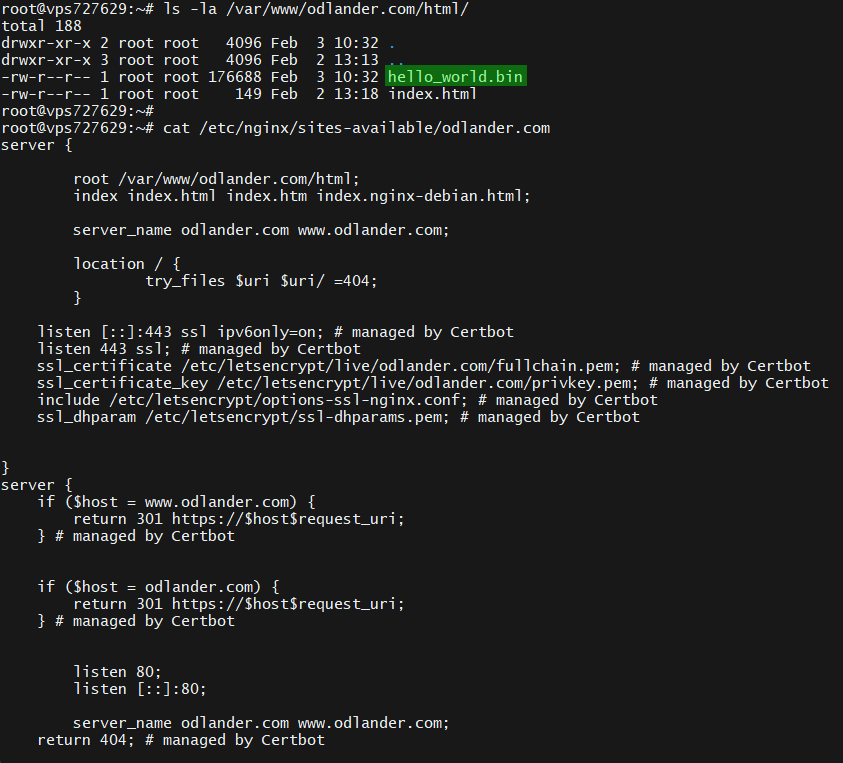
\includegraphics[width=0.8\linewidth]{figures/web_server.png}
  \caption{Web server}
  \label{fig:web_server}
\end{figure}

This also enables the possiblity for rollback to a previous firmware image in the event of a failed update \cite{espressif:esp-idf-programming-guide}. The \texttt{energy\_gateway\_ota} component stores the current firmware image version in the \texttt{ota\_data} partition. If the new firmware image fails to boot, the component could automatically rollback to the previous firmware image. This rollback functionality was not implemented in our project.

\subsubsection{UART communication}

\subsection{Concurrency}

When it comes to developing software with the Espressif IoT Development Framework (ESP-IDF), understanding the intricacies of priority levels is paramount for effective task management~\cite{Davis:2016}. The underlying operating system for ESP-IDF is FreeRTOS, which is a real-time operating system designed for microcontrollers that provides a multitasking environment for running multiple tasks simultaneously on a single processor. The priority-based preemptive scheduling algorithm employed by FreeRTOS is an essential feature that allows for efficient task management~\cite{espressif:esp-idf-programming-guide}.

ESP-IDF utilizes a range of 26 priority levels, numbered from 0 (highest) to 25 (lowest). The variable \texttt{ESP\_TASK\_PRIO\_MAX}, which represents the maximum allowed priority level in ESP-IDF, is currently set to 25 and can be found in the FreeRTOSConfig.h file\cite{espressif:freertosconfig}. This limitation ensures that the system remains stable and responsive, even when multiple high-priority tasks are running concurrently. By utilizing these priority levels effectively, developers can optimize system performance and ensure that critical tasks receive the necessary resources to execute efficiently~\cite{espressif:esp-idf-programming-guide}.

Choosing the appropriate priority level for a task requires careful consideration of its criticality and potential impact on the system. For instance, a high-priority task that reads data from a serial port demands immediate attention to avoid data loss or errors. In our project, we assigned a priority level of \texttt{ESP\_TASK\_PRIO\_MAX - 6} (level 19) to our serial-reading task. This priority level strikes a balance between prioritizing our task and allowing other tasks to run when needed. It also provides some headroom above the default priority levels of many other tasks in the system~\cite{espressif:esp-idf-programming-guide}, ensuring that our task receives immediate attention while still allowing for efficient resource allocation.

Moreover, it is worth noting that prioritization is not a one-size-fits-all solution. Different tasks have different criticality levels, and thus require different priority levels. Some tasks may be less critical but more time-consuming, while others may require frequent access to system resources. As such, the priority level should be carefully selected to ensure efficient task management and optimize system performance.

In conclusion, understanding the intricacies of priority levels is essential when programming with esp-idf. By choosing the appropriate priority level for each task, we can ensure efficient task management, avoid system performance degradation, and optimize system performance. With only 25 priority levels in ESP-IDF, developers have limited flexibility to assign priority levels based on the specific needs of their projects.

\subsection{Result}\label{sec:result}

\subsubsection{WiFi Provisioning through Bluetooth}

The WiFi provisioning through Bluetooth system was successfully developed and implemented on the ESP32 microcontroller. The system enables efficient configuration of WiFi credentials on ESP32 devices through the use of a BLE-enabled device. The system was tested, and it was found to be reliable and effective in provisioning WiFi credentials without the need for code modification. The system was integrated as a component using the ESP-IDF framework, enabling easy integration by other developers. The use of BLE-enabled devices enhances security, making it a potential solution in the realm of IoT.

\subsubsection{OTA Updates}

The OTA update system was successfully developed and implemented on the ESP32 microcontroller. The system allows for remote firmware updates of the ESP32 board via a Wi-Fi connection, eliminating the need for a physical connection. The system was tested, and it was found to be reliable and effective in updating the firmware image without interrupting any critical tasks that the unit may be currently running. The \texttt{energy\_gateway\_ota} component was utilized to handle the initialization, download, verification, and activation of new firmware images. The component also integrates git tags as a versioning system, resulting in the update being aborted if the tags differ. The system also enables the possibility for rollback to a previous firmware image in the event of a failed update. However, this rollback functionality was not implemented in our project.

\subsubsection{UART Communication}

The implementation of serial communication on the ESP32 microcontroller was successful. The microcontroller was connected to a Wireless Stick~\ref{fig:serial_connection} and able to establish a serial communication channel with the Stick, running MicroPython, to receive and transmit data. With the \texttt{uart\_read\_bytes(ECHO\_UART\_PORT\_NUM, (char *) uartData, (UART\_BUF\_SIZE - 1), 20 / portTICK\_PERIOD\_MS);} function call, bytes was read, with a timeout of 20 milliseconds, and placed in the \texttt{uartData} buffer. 

The Wireless Stick was configured to send random integers between 0 and 255 over serial that The ESP32 microcontroller was programmed to receive. The microcontroller was designed to send back a value of 1 if the received value was greater than 250 and a value of 0 if the value was less than 5. The UART communication was stress tested by sending data at 33Hz

When the data had been received and the buffer checked for the correct value, the buffer was cleared and the task yielded for 10 milliseconds, using \texttt{vTaskDelay(10 / portTICK\_PERIOD\_MS);}.

\begin{figure}[ht]
  \centering
  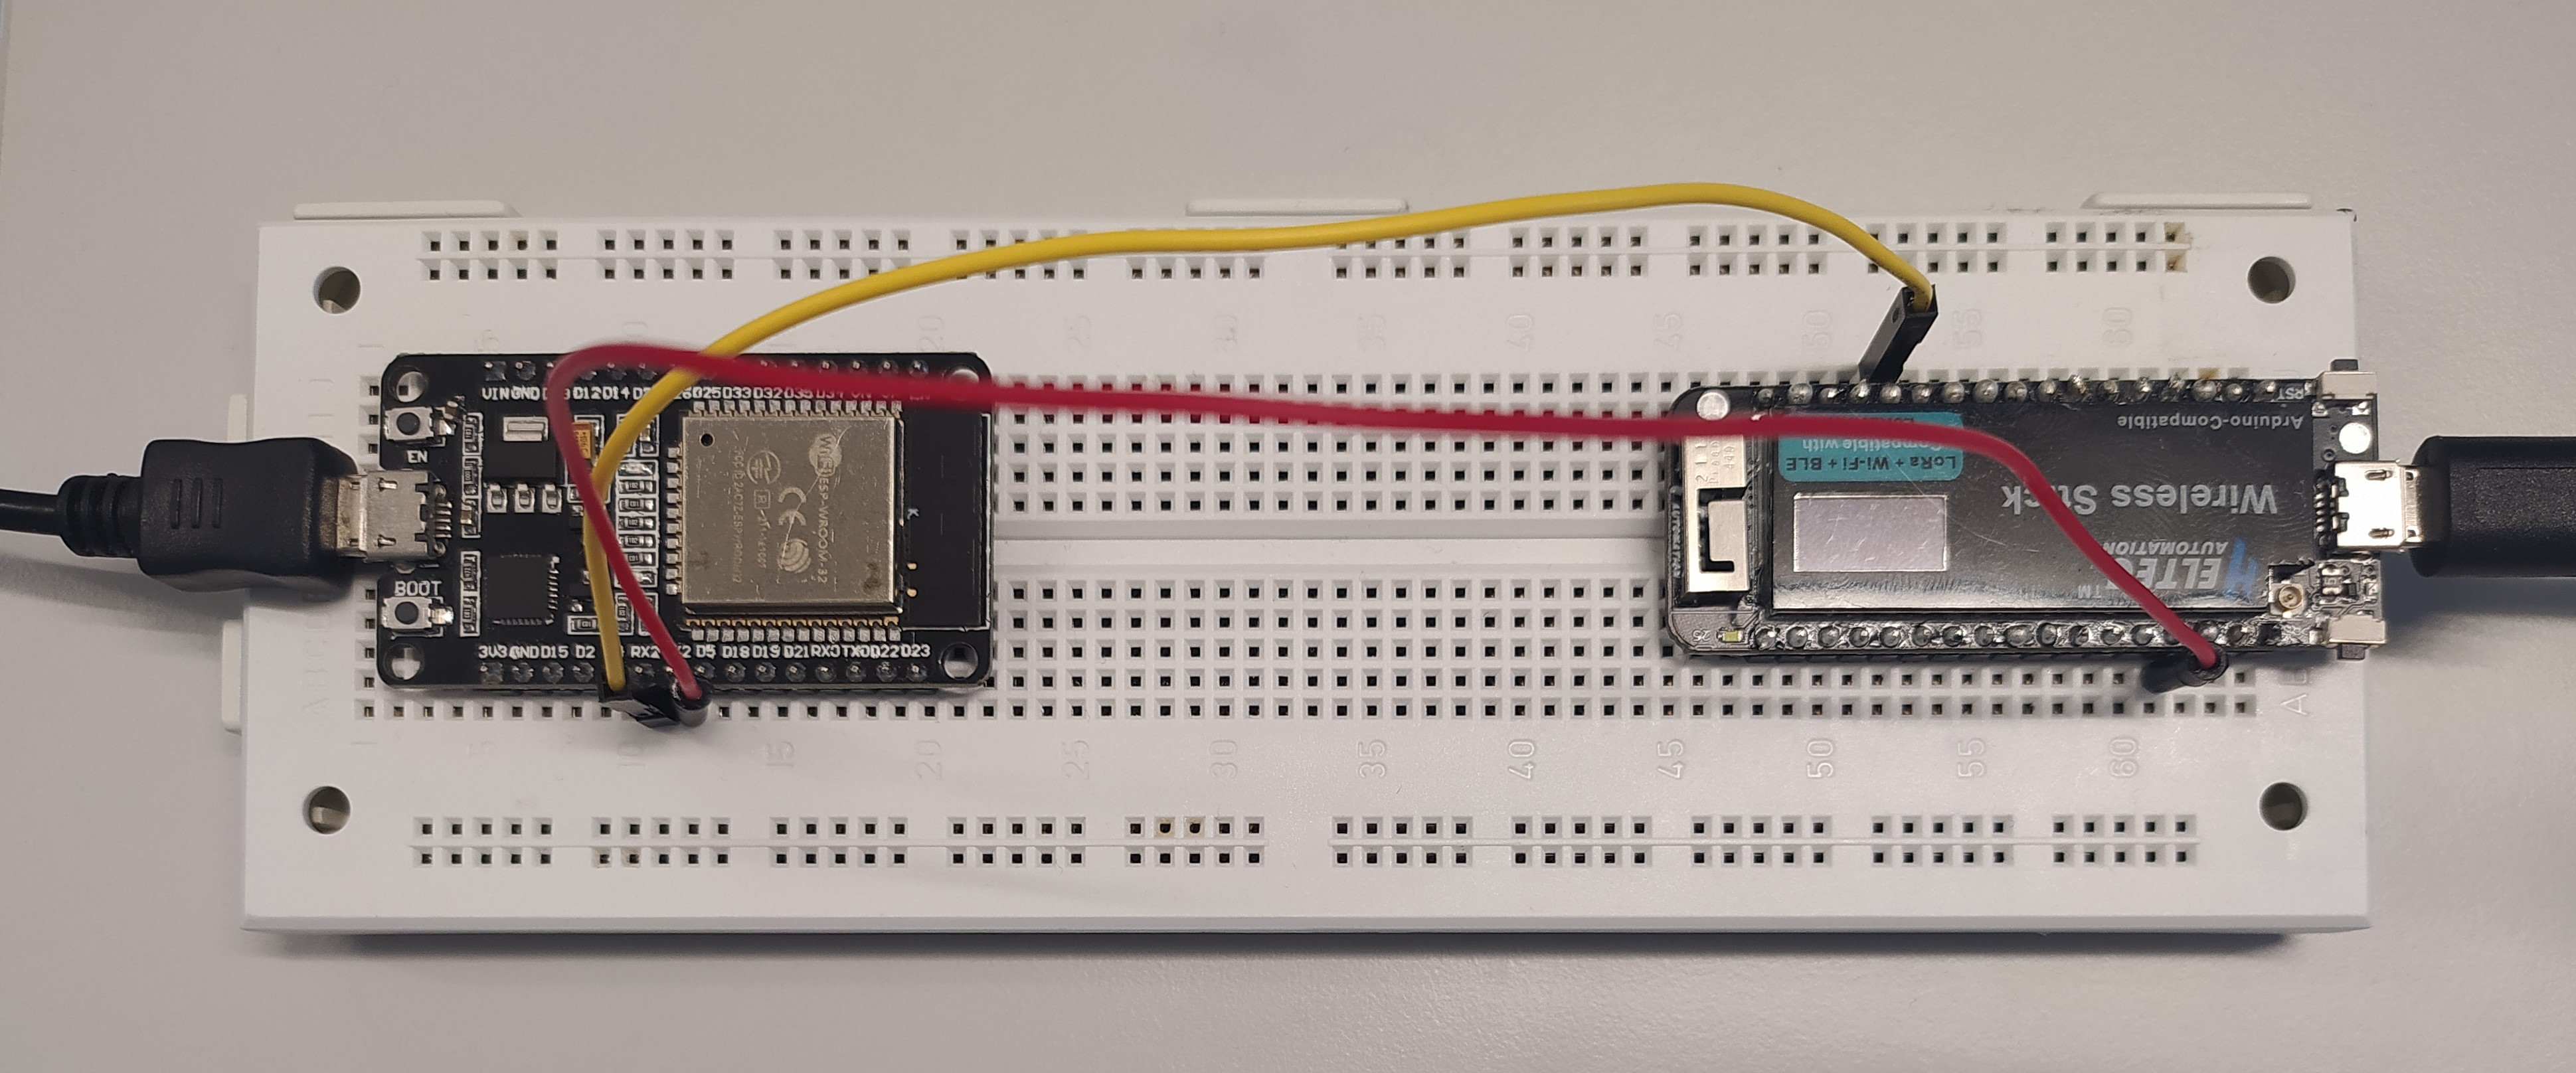
\includegraphics[width=0.8\linewidth]{figures/serial_connection.jpg}
  \caption{ESP32 connected via serial}
  \label{fig:serial_connection}
\end{figure}

\subsubsection{Concurrency}

\clearpage
%----------------------------------------------------------------------------------------
% Discussion
%----------------------------------------------------------------------------------------
\section{Discussion}
\label{sec:discussion}

\subsection{Evaluation}
\label{sec:evaluation}

We have successfully implemented and integrated three key features into the Energy Gateway. These features include WiFi provisioning through Bluetooth, OTA updates, and UART communication.

Our WiFi provisioning through Bluetooth feature allows for streamlined configuration of WiFi credentials on ESP32 devices using a BLE-enabled device, such as a smartphone. This feature provides a more efficient and secure method of communication between devices in the realm of IoT, making it a valuable addition to the Energy Gateway system.

The OTA update feature enables remote firmware updates of the ESP32 board via a Wi-Fi connection, eliminating the need for a physical connection. This feature allows for the easy deployment of updates to the Energy Gateway system, even when it is deployed in hard-to-reach locations. We have also implemented a versioning system based on git tags to ensure that only new firmware images are updated and avoid updating the firmware to an older version.

Our UART communication feature allows the Energy Gateway system to poll and send data to serial devices. We have successfully established a UART connection between the ESP32 microcontroller and a Heltec Wireless Stick, which simulates the behavior of a serial device. We have also tested the system's performance under stress conditions, which helps ensure that the feature functions reliably in the final Energy Gateway product.

In terms of the results, our work has shown that the features have been successfully implemented and tested. The WiFi provisioning through Bluetooth feature simplifies the process of configuring WiFi credentials on ESP32 devices and enhances security by using BLE-enabled devices. The OTA update feature eliminates the need for a physical connection and allows for easy deployment of updates to the Energy Gateway system, while the UART communication feature provides the capability to poll and send data to serial devices.

Overall, our work on the Energy Gateway system has resulted in a more efficient and capable product that can effectively monitor and control energy consumption in a building. The features implemented have the potential to enhance the usability and security of the system and enable easy deployment of updates, which is critical in the realm of IoT. We have also demonstrated our ability to program with the ESP-IDF framework and utilize the FreeRTOS real-time operating system effectively.

\subsubsection{Explanation}
\label{sec:explanation}

Our work on implementing three key features into the Energy Gateway has shown successful results. The WiFi provisioning through Bluetooth feature, which enables streamlined configuration of WiFi credentials on ESP32 devices, is a valuable addition to the Energy Gateway system. Previous research has shown that Bluetooth Low Energy (BLE) is a low-power communication protocol that is commonly used in IoT devices due to its low energy consumption and high security features //TODO: Add reference. The implementation of BLE in our system enhances security and improves the efficiency of communication between devices.

The OTA update feature, which enables remote firmware updates of the ESP32 board via a Wi-Fi connection, eliminates the need for a physical connection and simplifies the process of updating the system. Previous research has shown that OTA updates are critical for ensuring the security and reliability of IoT systems, as they allow for easy deployment of updates and patches to address vulnerabilities TODO: Add reference. Our implementation of OTA updates in the Energy Gateway system is an important step towards ensuring the security and reliability of the system.

The UART communication feature, which enables the Energy Gateway system to poll and send data to serial devices, is another important addition to the system. Previous research has shown that UART communication is a common method used in IoT systems for inter-device communication due to its simplicity and reliability TODO: Add reference. Our successful implementation of UART communication in the Energy Gateway system shows that we are well-versed in the fundamental principles of IoT communication protocols.

\subsubsection{Limitations and possible sources of errors}
\label{sec:limitations}
\clearpage
%----------------------------------------------------------------------------------------
% Conclusion
%----------------------------------------------------------------------------------------
\section{Conclusion}
\label{sec:conclusion}

\clearpage

%----------------------------------------------------------------------------------------
%	BIBLIOGRAPHY
%----------------------------------------------------------------------------------------
\renewcommand{\refname}{\spacedlowsmallcaps{References}} % For modifying the bibliography heading

\bibliographystyle{unsrt}

\bibliography{bibliography.bib} % The file containing the bibliography

%----------------------------------------------------------------------------------------

\end{document}